\documentclass[10pt,a4paper,twocolumn]{article}

\newcommand{\projecttitle}{Is the closing-auction imbalance already in the price?
  Evidence from 5.2 million Nasdaq auction snapshots}

\usepackage{iftex}
\ifPDFTeX
  \usepackage[T1]{fontenc}
  \usepackage[utf8]{inputenc}
  \IfFileExists{carlito.sty}%
    {\usepackage[sfdefault]{carlito}}%
    {\usepackage[scaled=0.92]{helvet}\renewcommand{\familydefault}{\sfdefault}}%
  \usepackage{courier}
\else
  \usepackage[no-math]{fontspec}
  \setmainfont{Carlito}[Extension=.ttf, UprightFont=*-Regular, BoldFont=*-Bold,
    ItalicFont=*-Italic, BoldItalicFont=*-BoldItalic]
\fi

\usepackage[margin=18mm,bottom=20mm,columnsep=7mm]{geometry}
\usepackage{amsmath}
\usepackage{xcolor}
\usepackage{graphicx}
\usepackage{tabularx}
\usepackage{array}
\usepackage{booktabs}
\usepackage{enumitem}
\usepackage{titlesec}
\usepackage{needspace}
\usepackage[font=small,labelfont=bf]{caption}
\usepackage[hidelinks]{hyperref}
\hypersetup{pdftitle={\projecttitle},
            pdfsubject={CSE558 Data Science, Monsoon 2026: Midterm Project Report}}

\titleformat{\section}{\normalfont\large\bfseries}{\thesection.}{0.5em}{}
\titlespacing*{\section}{0pt}{12pt}{3pt}
\titleformat{\subsection}{\normalfont\normalsize\bfseries}{\thesubsection}{0.5em}{}
\titlespacing*{\subsection}{0pt}{10pt}{2pt}
\newcommand{\sectionbreak}{\needspace{10\baselineskip}}
\newcommand{\subsectionbreak}{\needspace{10\baselineskip}}

\setlength{\parindent}{0pt}
\setlength{\parskip}{4pt}
\setlist{leftmargin=1.2em, itemsep=2pt, topsep=2pt, parsep=0pt}
\renewcommand{\arraystretch}{1.25}
\setlength{\tabcolsep}{4pt}
\newcolumntype{L}[1]{>{\raggedright\arraybackslash}p{#1}}
\newcolumntype{Y}{>{\raggedright\arraybackslash}X}
\newcolumntype{K}[1]{>{\raggedright\arraybackslash\bfseries\boldmath}p{#1}}

\newcommand{\field}[2]{\textbf{#1}~#2\par}
\newcommand{\tpart}[2]{\par\needspace{12\baselineskip}\smallskip\textbf{#1)~#2}\par}
\newcommand{\minihead}[1]{\par\needspace{8\baselineskip}\smallskip\textbf{#1}\par}
\newcommand{\code}[1]{\texttt{#1}}

\graphicspath{{../figures/}}
\newcommand{\nRawRows}{5{,}237{,}980}
\newcommand{\nRawCols}{17}
\newcommand{\nRawCells}{89{,}045{,}660}
\newcommand{\nCleanRows}{5{,}237{,}760}
\newcommand{\nEncCols}{223}
\newcommand{\nEncCells}{1{,}168{,}020{,}480}
\newcommand{\nEncNumeric}{13}
\newcommand{\nEncEngineered}{5}
\newcommand{\nStocks}{200}
\newcommand{\nDays}{481}
\newcommand{\nMemBefore}{934}
\newcommand{\nMemAfter}{400}
\newcommand{\nMissingBefore}{5{,}752{,}930}
\newcommand{\nMissingAfter}{5{,}751{,}289}
\newcommand{\nEmptyRows}{220}
\newcommand{\nStructuralRows}{2{,}856{,}960}
\newcommand{\nFarOutliers}{207}
\newcommand{\nWinsorRows}{10{,}475}
\newcommand{\nWinsorLow}{-49.4}
\newcommand{\nWinsorHigh}{51.8}
\newcommand{\nFenceIqr}{32.5\%}
\newcommand{\nFenceIqrThree}{25.8\%}
\newcommand{\nFenceMad}{25.0\%}
\newcommand{\nFenceSigma}{0.12\%}
\newcommand{\nFenceCheb}{0.009\%}
\newcommand{\nStockDaysPresent}{95{,}232}
\newcommand{\nStockDaysMissing}{968}
\newcommand{\nStocksWithGaps}{15}
\newcommand{\nMaxMissingDays}{295}
\newcommand{\nIndexUnexplained}{$2.1\times10^{-8}$}
\newcommand{\nIndexWeightSum}{1.0000}
\newcommand{\nIndexWeightMax}{0.040}
\newcommand{\nIndexResidSd}{0.005}
\newcommand{\nTargetSd}{9.5}
\newcommand{\nTargetKurt}{22.6}
\newcommand{\nTargetSkew}{0.20}
\newcommand{\nSpreadMedian}{3.69}
\newcommand{\nTailObserved}{1.49\%}
\newcommand{\nTailNormal}{0.27\%}
\newcommand{\nTailCheb}{11.1\%}
\newcommand{\nTailRatio}{5.5}
\newcommand{\nEmptyNoTarget}{88}
\newcommand{\nStockDaysBefore}{95{,}236}
\newcommand{\nStructuralCells}{5{,}713{,}920}
\newcommand{\nFarPostMissing}{37{,}162}
\newcommand{\nGofChi}{98{,}064}
\newcommand{\nGofDf}{17}
\newcommand{\nAcfOne}{0.78}
\newcommand{\nAcfFive}{0.11}
\newcommand{\nAcfSix}{-0.06}
\newcommand{\nFlagSell}{40\%}
\newcommand{\nFlagBuy}{39\%}
\newcommand{\nFlagNone}{22\%}
\newcommand{\nBalancedPre}{13\%}
\newcommand{\nBalancedPost}{25\%}
\newcommand{\nSdm}{1.85}
\newcommand{\nTestRows}{952{,}320}
\newcommand{\nOneEst}{0.47}
\newcommand{\nOneCi}{0.44 to 0.49}
\newcommand{\nOneT}{32.5}
\newcommand{\nOneDf}{480}
\newcommand{\nOneP}{$8.0\times10^{-124}$}
\newcommand{\nOneRawEst}{0.48}
\newcommand{\nOneRawCi}{0.45 to 0.51}
\newcommand{\nOneBootCi}{0.44 to 0.49}
\newcommand{\nOneNaiveZ}{42.0}
\newcommand{\nOneNaiveN}{738{,}083}
\newcommand{\nOneOverlapN}{4{,}106{,}317}
\newcommand{\nOneWelchT}{41.9}
\newcommand{\nOneWelchDiff}{0.93}
\newcommand{\nOneVarRatio}{1.09}
\newcommand{\nOnePositiveDays}{458}
\newcommand{\nOneShareOfSdm}{27\%}
\newcommand{\nTwoChi}{33.2}
\newcommand{\nTwoDf}{2}
\newcommand{\nTwoP}{$6.1\times10^{-8}$}
\newcommand{\nTwoN}{95{,}193}
\newcommand{\nTwoV}{0.019}
\newcommand{\nTwoVThreshold}{0.10}
\newcommand{\nTwoMinExpected}{6{,}020}
\newcommand{\nTwoUpBuy}{50.4\%}
\newcommand{\nTwoUpSell}{48.4\%}
\newcommand{\nTwoDiff}{2.0}
\newcommand{\nTwoDiffCi}{1.3 to 2.7}
\newcommand{\nTwoPropZ}{5.73}
\newcommand{\nTwoG}{33.2}
\newcommand{\nTwoDayT}{3.62}
\newcommand{\nTwoDayP}{$1.6\times10^{-4}$}
\newcommand{\nTwoAllChi}{1{,}233}
\newcommand{\nTwoAllN}{951{,}770}
\newcommand{\nThreeEst}{0.047}
\newcommand{\nThreeCi}{0.040 to 0.054}
\newcommand{\nThreeT}{13.6}
\newcommand{\nThreeDf}{480}
\newcommand{\nThreeP}{$7.8\times10^{-36}$}
\newcommand{\nThreeThreshold}{0.02}
\newcommand{\nThreePre}{0.032}
\newcommand{\nThreePreCi}{0.028 to 0.037}
\newcommand{\nThreePost}{0.080}
\newcommand{\nThreePostCi}{0.076 to 0.084}
\newcommand{\nThreeRatio}{2.5}
\newcommand{\nThreeFisherZ}{20.5}
\newcommand{\nThreeSignDays}{363}
\newcommand{\nThreeSignP}{$4.8\times10^{-30}$}
\newcommand{\nThreeWilcoxonP}{$2.2\times10^{-33}$}
\newcommand{\nThreePooledPre}{0.030}
\newcommand{\nThreePooledPost}{0.072}
\newcommand{\nThreePooledPreT}{20.8}
\newcommand{\nThreePooledPostT}{49.8}
\newcommand{\nFourF}{0.771}
\newcommand{\nFourCi}{0.766 to 0.775}
\newcommand{\nFourDf}{476{,}159}
\newcommand{\nFourP}{$<10^{-300}$}
\newcommand{\nFourSdPre}{10.5}
\newcommand{\nFourSdPost}{9.2}
\newcommand{\nFourKurtPre}{21}
\newcommand{\nFourKurtPost}{24}
\newcommand{\nFourBf}{3{,}954}
\newcommand{\nFourBfP}{$<10^{-300}$}
\newcommand{\nFourDayRatio}{0.79}
\newcommand{\nFourDayRatioCi}{0.77 to 0.80}
\newcommand{\nFourDayT}{-24.5}
\newcommand{\nFourWinsF}{0.779}
\newcommand{\nFourLow}{0.90}
\newcommand{\nFourHigh}{1.11}
\newcommand{\nFourDrop}{23\%}
\newcommand{\nFiveN}{738{,}083}
\newcommand{\nFiveEst}{39.2\%}
\newcommand{\nFiveCi}{39.1 to 39.3}
\newcommand{\nFiveZ}{-185.4}
\newcommand{\nFiveP}{$1.000$}
\newcommand{\nFiveGross}{52.0\%}
\newcommand{\nFiveNet}{-2.40}
\newcommand{\nFiveThreshold}{52\%}
\newcommand{\nFiveDayT}{-133.0}
\newcommand{\nBoundT}{0.028}
\newcommand{\nBoundCheb}{0.064}
\newcommand{\nBoundHoeff}{6.42}
\newcommand{\nBoundChebRatio}{2.3}
\newcommand{\nBoundHoeffRatio}{228}
\newcommand{\nBoundTCi}{0.44 to 0.49}
\newcommand{\nBoundChebCi}{0.40 to 0.53}
\newcommand{\nBoundHoeffCi}{-6.0 to 6.9}
\newcommand{\nBoundRange}{51.8}
\newcommand{\nJumpReal}{0.057}
\newcommand{\nJumpRealCi}{0.040 to 0.074}
\newcommand{\nJumpLast}{0.193}
\newcommand{\nJumpLastCi}{0.181 to 0.206}
\newcommand{\nJumpFour}{0.084}
\newcommand{\nJumpTwo}{0.054}
\newcommand{\nJumpSevenMin}{-0.082}
\newcommand{\nIcBeforeBoundary}{-0.037}
\newcommand{\nIcAtBoundary}{0.108}
\newcommand{\nIcLast}{0.247}
\newcommand{\nIcMin}{-0.064}
\newcommand{\nSensWith}{0.054}
\newcommand{\nSensWithCi}{0.047 to 0.060}
\newcommand{\nSensWithout}{0.014}
\newcommand{\nSensWithoutCi}{0.006 to 0.021}
\newcommand{\nRobPositive}{11}
\newcommand{\nRobTotal}{11}
\newcommand{\nPermOneP}{$5.0\times10^{-4}$}
\newcommand{\nPermOneMax}{0.039}
\newcommand{\nPermOneN}{2{,}000}
\newcommand{\nFlipThreeP}{$1.0\times10^{-4}$}
\newcommand{\nFlipThreeMax}{0.014}
\newcommand{\nFlipThreeN}{10{,}000}
\newcommand{\nFinalGross}{2.40}
\newcommand{\nFinalHalf}{1.92}
\newcommand{\nFinalNet}{0.48}
\newcommand{\nFinalNetCi}{0.39 to 0.58}
\newcommand{\nFinalT}{9.7}
\newcommand{\nFinalHit}{52.7\%}
\newcommand{\nFinalFirst}{0.74}
\newcommand{\nFinalSecond}{0.23}
\newcommand{\nFinalSecondCi}{0.10 to 0.36}
\newcommand{\nStrongGross}{1.77}
\newcommand{\nStrongHalf}{3.81}
\newcommand{\nStrongNet}{-1.99}
\newcommand{\nStrongNetCi}{-2.18 to -1.79}
\newcommand{\nBreakPre}{0.30}
\newcommand{\nBreakPost}{0.71}
\newcommand{\nTFitDf}{3.1}
\newcommand{\nTFitScale}{6.2}
\newcommand{\nTFitChi}{568}
\newcommand{\nTFitGain}{0.125}
\newcommand{\nNormChi}{98{,}064}
\newcommand{\nFlipMean}{2.69}
\newcommand{\nFlipVar}{6.59}
\newcommand{\nFlipDispersion}{2.45}
\newcommand{\nFlipZero}{19.6\%}
\newcommand{\nFlipZeroPoisson}{6.8\%}
\newcommand{\nFlipChi}{189{,}527}
\newcommand{\nFlipDf}{10}
\newcommand{\nMidOneEst}{0.31}
\newcommand{\nMidOneCi}{0.28 to 0.35}
\newcommand{\nMidOneT}{19.7}
\newcommand{\nWapOneEst}{0.31}
\newcommand{\nMidOneRetained}{101\%}
\newcommand{\nMidFiveHit}{37.3\%}
\newcommand{\nWapFiveHit}{38.0\%}
\newcommand{\nCmItems}{95{,}232}
\newcommand{\nCmCounters}{14{,}000}
\newcommand{\nCmWidth}{2{,}000}
\newcommand{\nCmDepth}{7}
\newcommand{\nCmWithin}{100\%}
\newcommand{\nCmMaxShare}{66\%}
\newcommand{\nCmTop}{9}
\newcommand{\nCmMemory}{15\%}
\newcommand{\nMdeOne}{0.036}
\newcommand{\nDaysOne}{1}
\newcommand{\nThrOne}{1.85}
\newcommand{\nMdeThree}{0.010}
\newcommand{\nDaysThree}{115}
\newcommand{\nThrThree}{0.02}
\newcommand{\nMdeFour}{0.027}
\newcommand{\nDaysFour}{32}
\newcommand{\nThrFour}{0.105}
\newcommand{\nMdeFive}{0.002}
\newcommand{\nDaysFive}{5}
\newcommand{\nThrFive}{0.02}
\newcommand{\nMdeOneRatio}{52}
\newcommand{\nRobRows}{first half of days & 0.024 & 0.087 & +0.063 (0.054 to 0.072) \\
second half of days & 0.041 & 0.073 & +0.031 (0.022 to 0.041) \\
size: low & 0.050 & 0.080 & +0.029 (0.021 to 0.037) \\
size: mid & 0.033 & 0.075 & +0.041 (0.032 to 0.051) \\
size: high & 0.016 & 0.098 & +0.081 (0.071 to 0.091) \\
spread: low & 0.016 & 0.094 & +0.078 (0.069 to 0.088) \\
spread: mid & 0.035 & 0.073 & +0.038 (0.028 to 0.047) \\
spread: high & 0.046 & 0.082 & +0.036 (0.028 to 0.043) \\
day volatility: low & 0.038 & 0.077 & +0.039 (0.029 to 0.050) \\
day volatility: mid & 0.032 & 0.080 & +0.048 (0.036 to 0.059) \\
day volatility: high & 0.028 & 0.082 & +0.055 (0.041 to 0.068) \\}
\newcommand{\nJumpRows}{15:50:00 to 15:51:00 & -0.019 & -0.032 to -0.006 \\
15:51:00 to 15:52:00 & +0.054 & 0.043 to 0.066 \\
15:52:00 to 15:53:00 & +0.010 & -0.002 to 0.022 \\
15:53:00 to 15:54:00 & -0.006 & -0.019 to 0.007 \\
15:54:00 to 15:55:00 & +0.057 & 0.040 to 0.074 \\
15:55:00 to 15:56:00 & -0.056 & -0.071 to -0.041 \\
15:56:00 to 15:57:00 & -0.082 & -0.094 to -0.070 \\
15:57:00 to 15:58:00 & +0.084 & 0.073 to 0.096 \\
15:58:00 to 15:59:00 & +0.193 & 0.181 to 0.206 \\}
\newcommand{\nSixEst}{0.140}
\newcommand{\nSixCi}{0.134 to 0.146}
\newcommand{\nSixT}{46.9}
\newcommand{\nSixDf}{179}
\newcommand{\nSixP}{$8.4\times10^{-103}$}
\newcommand{\nSixPerm}{$1.0\times10^{-4}$}
\newcommand{\nSixThreshold}{0.01}
\newcommand{\nSixMlp}{0.192}
\newcommand{\nSixBase}{0.052}
\newcommand{\nSixRatio}{3.7}
\newcommand{\nSixTestDays}{180}
\newcommand{\nSixTrainRows}{2{,}600{,}950}
\newcommand{\nSixTestRows}{359{,}960}
\newcommand{\nSixFeatures}{19}
\newcommand{\nLgbmIc}{0.200}
\newcommand{\nLgbmGain}{0.148}
\newcommand{\nLgbmGainCi}{0.142 to 0.153}
\newcommand{\nMlpLgbm}{-0.008}
\newcommand{\nMlpLgbmCi}{-0.009 to -0.006}
\newcommand{\nGruIc}{0.195}
\newcommand{\nSnapIc}{0.172}
\newcommand{\nGruGain}{0.022}
\newcommand{\nGruGainCi}{0.020 to 0.025}
\newcommand{\nDmZeroT}{17.1}
\newcommand{\nDmLinT}{16.9}
\newcommand{\nDmLinP}{$2.4\times10^{-39}$}
\newcommand{\nSeedSdMlp}{0.0010}
\newcommand{\nSeedSdLgbm}{0.0004}
\newcommand{\nSeedSdGru}{0.0022}
\newcommand{\nSeedRatio}{145}
\newcommand{\nMidGain}{-0.010}
\newcommand{\nMidGainCi}{-0.016 to -0.003}
\newcommand{\nMidMlp}{0.031}
\newcommand{\nMidBase}{0.040}
\newcommand{\nMidShare}{-7\%}
\newcommand{\nSelNet}{0.68}
\newcommand{\nSelNetCi}{0.58 to 0.77}
\newcommand{\nSelT}{13.6}
\newcommand{\nSelHit}{53.5\%}
\newcommand{\nSelShare}{13.5\%}
\newcommand{\nSelTrades}{48{,}534}
\newcommand{\nSelMidNet}{-0.40}
\newcommand{\nSelMidNetCi}{-0.51 to -0.28}
\newcommand{\nSelMidHit}{46.8\%}
\newcommand{\nSelMidT}{-6.9}
\newcommand{\nSelMidP}{$1.000$}
\newcommand{\nCtAcc}{82.3\%}
\newcommand{\nCtZ}{388}
\newcommand{\nCtN}{359{,}960}
\newcommand{\nCtDayCi}{82.0 to 82.7}
\newcommand{\nImpFirst}{depth imbalance}
\newcommand{\nImpFirstShare}{19\%}
\newcommand{\nImpSecond}{spread bps}
\newcommand{\nImpThird}{ref gap bps}
\newcommand{\nImpImbShare}{5\%}
\newcommand{\nHolmOne}{$4.0\times10^{-123}$}
\newcommand{\nHolmTwo}{$1.2\times10^{-7}$}
\newcommand{\nHolmThree}{$2.3\times10^{-35}$}
\newcommand{\nHolmFour}{$<10^{-300}$}
\newcommand{\nHolmFive}{$1.000$}
\newcommand{\nHolmSix}{$3.4\times10^{-102}$}


\begin{document}

\twocolumn[%
{\small\bfseries CSE558 Data Science\ \ \textbullet\ \ Midterm Project Report\ \ \textbullet\ \ Monsoon 2026\par}
\vspace{4pt}
{\LARGE\bfseries\raggedright\projecttitle\par}
\vspace{6pt}
\rule{\linewidth}{1pt}

{\small
\begin{tabularx}{\linewidth}{@{}K{2.4cm} Y@{}}
\toprule
Group name & Closing Cross \\
Dataset & kaggle.com/competitions/optiver-trading-at-the-close (file \code{train.csv}) \\
Code & github.com/USERNAME/nasdaq-closing-cross (code, README and supplement) \\
\bottomrule
\end{tabularx}}

\vspace{2pt}
{\small
\begin{tabularx}{\linewidth}{@{}L{0.5cm} L{3.4cm} L{2.3cm} L{4.8cm} Y@{}}
\toprule
\textbf{\#} & \textbf{Name} & \textbf{Roll no.} & \textbf{Institute email} & \textbf{Contribution} \\
\midrule
1 & Arush Gumber & 2023136 & arush23136@iiitd.ac.in & Problem statement, Tests 3 to 5, code (4, 5) \\
2 & Aditri Jain & 2024027 & aditri24027@iiitd.ac.in & Dataset and size check (1) \\
3 & Arnesh Batra & 2023129 & arnesh23129@iiitd.ac.in & Preparation, before and after (2, 3) \\
4 & Anika Goyal & 2024072 & anika24072@iiitd.ac.in & EDA, Tests 1 and 2 (4, 5) \\
5 & Akshainie Rawat & 2024054 & akshainie24054@iiitd.ac.in & Limitations, README, report (5, 6) \\
\bottomrule
\end{tabularx}}
\vspace{12pt}
]

\section{Dataset}

\field{Source:}{Optiver, ``Trading at the Close'', a Kaggle competition released in 2023. It records the last ten
minutes of the Nasdaq closing auction, the call auction that sets each stock's official closing price at 16:00, for
\nStocks{} stocks over \nDays{} trading days. One row is one stock at one 10-second snapshot between 15:50 and
15:59.}

\field{What is raw about it:}{the indicative clearing prices are missing for half the rows by exchange rule; four
stock-days carry no book at all; far prices reach hundreds of times the reference price; \nStocksWithGaps{} stocks
leave and re-enter the panel; the response is a 60-second move sampled every 10 seconds, so consecutive rows share
most of their window; and the index that the response is measured against is hidden.}

{\small
\begin{tabularx}{\linewidth}{@{}L{3.0cm} Y Y@{}}
\toprule
 & \textbf{Raw file} & \textbf{After encoding} \\
\midrule
Instances (rows) & \nRawRows & \nCleanRows \\
Attributes (columns) & \nRawCols & \nEncCols \\
Instances $\times$ attributes & \nRawCells & \nEncCells \\
\bottomrule
\end{tabularx}}

\field{Size check:}{the raw file alone gives $\nRawRows\times\nRawCols=\nRawCells\ge3{,}000{,}000$. After
cleaning we keep \nEncNumeric{} numeric columns, add \nEncEngineered{} engineered ones and one-hot encode the stock
(200 levels), the imbalance side (3) and the auction phase (2), which gives
$\nCleanRows\times\nEncCols=\nEncCells$.}

\minihead{Key features}
{\footnotesize
\begin{tabularx}{\linewidth}{@{}L{3.3cm} L{1.3cm} Y@{}}
\toprule
\textbf{Feature} & \textbf{Type} & \textbf{Real-world meaning} \\
\midrule
\code{target} & continuous & the stock's 60\,s return minus the index's 60\,s return, in basis points (1 bp $=0.01\%$); our response \\
\code{imbalance\_size} & continuous & shares that would be left unmatched if the auction cleared now \\
\code{imbalance\_buy\_}\allowbreak\code{sell\_flag} & nominal & side of that imbalance: buy, sell or none \\
\code{matched\_size} & continuous & shares that would trade at the current reference price \\
\code{reference\_price} & continuous & the price at which the auction would clear now \\
\code{near/far\_price} & continuous & indicative clearing prices with and without the continuous book; published from 15:55 \\
\code{bid/ask\_price} & continuous & best quotes in the continuous market \\
\code{seconds\_in\_bucket} & discrete & seconds since 15:50 (0 to 540) \\
\code{signed\_imbalance} & engineered & side $\times$ imbalance\,/\,matched shares: $+0.3$ means buyers want 30\% more
shares than are matched, $-0.3$ the same for sellers \\
\bottomrule
\end{tabularx}}

\section{Data preparation}

Every step below was fixed before any hypothesis test was run, and each records its row counts.

{\footnotesize
\begin{tabularx}{\linewidth}{@{}L{1.9cm} L{2.2cm} Y@{}}
\toprule
\textbf{Issue found} & \textbf{What we did} & \textbf{Why, and not the alternative} \\
\midrule
\nEmptyRows{} rows (4 stock-days) with no book at all
 & dropped
 & no market existed for that stock that day; \nEmptyNoTarget{} of these rows also lack the target, so imputing would
   invent both \\
Near and far price missing in \nStructuralRows{} rows before 15:55
 & kept missing; added a phase flag
 & the exchange publishes them only from 15:55. Imputing would hand the analysis information no trader had \\
Far prices hundreds of times the reference
 & \nFarOutliers{} values beyond 10 sd set to missing
 & Tukey and MAD fences flag a quarter of all far prices (Figure~\ref{fig:fences}), because the far price spreads out
   as the imbalance grows: that is economics, not error. Chebyshev guarantees a 10 sd fence flags at most 1\% under
   any distribution \\
Far price missing in \nFarPostMissing{} rows after 15:55
 & kept missing
 & it needs auction-only interest on both sides; no test uses it \\
Target with excess kurtosis \nTargetKurt{}
 & winsorised copy at 0.1\% and 99.9\% (\nWinsorLow{} and \nWinsorHigh{} bps); raw kept
 & extreme moves are real in an auction, so no row is deleted. Mean-based tests use the clipped copy and report the
   raw result beside it \\
60\,s targets sampled every 10\,s
 & tests use one snapshot per minute
 & neighbouring targets share up to 50 of their 60 seconds (Figure~\ref{fig:acf}); every row would inflate the sample
   about sixfold \\
Hidden index behind the target
 & recovered by least squares
 & the implied index return is the same for every stock at a timestamp (median spread \nIndexResidSd{} bps), and 200
   positive weights summing to \nIndexWeightSum{} reproduce it with unexplained variance \nIndexUnexplained. The
   response is what it claims to be \\
Sizes and prices not comparable across stocks
 & engineered signed imbalance, spread and near/far gaps in bps
 & a 1M-share imbalance is large for a small stock and noise for a large one \\
Side coded $-1,0,1$; 200 stock ids
 & one-hot encoded
 & an integer code would make ``sell $<$ none $<$ buy'' a magnitude \\
Duplicate keys
 & checked on (stock, day, second)
 & none found \\
\bottomrule
\end{tabularx}}

\begin{figure}[!t]
  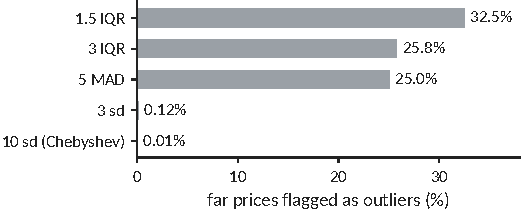
\includegraphics[width=\linewidth]{fig_outlier_fences}
  \caption{Quartile-based fences would discard a quarter of all far prices. The Chebyshev fence removes only
  physically impossible values. Bars show the share of far prices each rule calls an outlier.}
  \label{fig:fences}
\end{figure}


\minihead{Processing at stream scale}
To total the imbalance of each of the \nCmItems{} stock-days in one pass, as a live feed would require, we streamed
every row through a Count-Min sketch with \nCmMemory{} of the memory of exact counting. Every estimate stayed within
the sketch's $\varepsilon N$ guarantee, and \nCmTop{} of the 10 heaviest stock-days were found.

\section{What changed after preparation}

{\footnotesize
\begin{tabularx}{\linewidth}{@{}L{3.1cm} L{1.6cm} Y@{}}
\toprule
\textbf{Measure} & \textbf{Before} & \textbf{After} \\
\midrule
Rows & \nRawRows & \nCleanRows \\
Stock-days present (of 96{,}200) & \nStockDaysBefore & \nStockDaysPresent \\
Missing cells & \nMissingBefore & \nMissingAfter{} (\nStructuralCells{} by exchange rule) \\
Impossible far prices & \nFarOutliers & 0 \\
Memory & \nMemBefore{} MB & \nMemAfter{} MB \\
Rows used per test & every snapshot & \nTestRows{} (one per minute) \\
\bottomrule
\end{tabularx}}

Cleaning removed almost no data: only \nEmptyRows{} rows went. What changed is the unit of analysis. The
autocorrelation of the target follows the overlap of its windows and vanishes at exactly one minute
(Figure~\ref{fig:acf}), so the honest sample is one snapshot per minute. Across days, \nStockDaysMissing{} stock-days
are absent; one stock is missing for \nMaxMissingDays{} days, so every comparison is made within a day.

\begin{figure}[!t]
  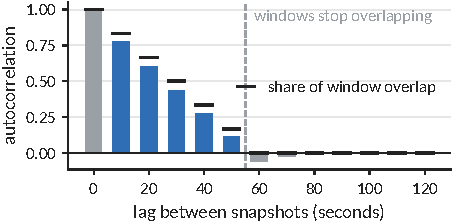
\includegraphics[width=\linewidth]{fig_autocorrelation}
  \caption{Consecutive targets are correlated only because their windows overlap. Bars are the correlation between a
  target and the one $k$ seconds later; black ticks are the share of the 60\,s window the two have in common. Both
  reach zero at 60\,s, so tests use one snapshot per minute.}
  \label{fig:acf}
\end{figure}

\section{Basic questions and problem statements}

\minihead{Basic questions}
\begin{enumerate}[label=\arabic*.]
  \item \textbf{How lopsided are auctions?} Sell imbalances appear in \nFlagSell{} of snapshots, buy in \nFlagBuy{},
  and \nFlagNone{} are balanced.
  \item \textbf{How costly is trading near the close?} The median quoted spread is \nSpreadMedian{} bps, and it
  narrows as 16:00 approaches (Figure~\ref{fig:profile}).
  \item \textbf{Is the target normal?} No (Figure~\ref{fig:dist}). Moves beyond 3 sd occur in \nTailObserved{} of
  rows, \nTailRatio{} times the normal \nTailNormal{} but inside Chebyshev's limit of \nTailCheb. A Student $t$ fitted
  by maximum likelihood has only \nTFitDf{} degrees of freedom: the variance exists, so the CLT and Chebyshev apply,
  but the fourth moment does not. It cuts the $\chi^2$ goodness-of-fit statistic from \nNormChi{} (normal) to
  \nTFitChi{}, yet is still rejected at this sample size.
  \item \textbf{Do imbalances change side at random?} No. A stock flips side \nFlipMean{} times a day on average, but
  the variance is \nFlipDispersion{} times the mean, and \nFlipZero{} of stock-days never flip against \nFlipZeroPoisson{}
  under a Poisson; $\chi^2=\nFlipChi$ on \nFlipDf{} d.f. Some auctions are one-sided all along, others churn.
\end{enumerate}

\begin{figure}[!t]
  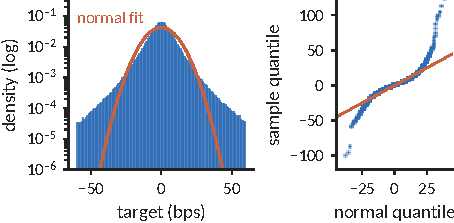
\includegraphics[width=\linewidth]{fig_target_distribution}
  \caption{The target is far more peaked and heavy-tailed than a normal. Left: histogram on a log scale, with the
  normal of the same mean and spread in orange; the bars sit far above it in both tails. Right: Q-Q plot; normal data
  would lie on the line. So tests average to one value per day and rely on the CLT across days.}
  \label{fig:dist}
\end{figure}

\begin{figure}[!t]
  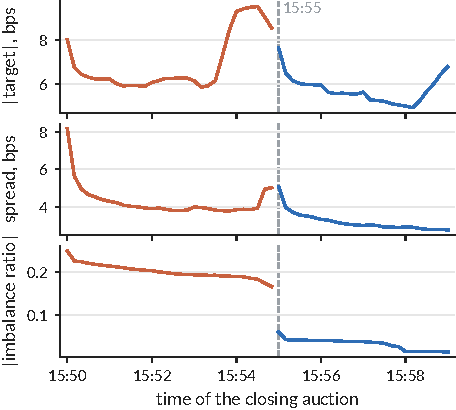
\includegraphics[width=\linewidth]{fig_auction_profile}
  \caption{The auction changes regime at 15:55. Each line is an average over all stocks and days at each 10\,s
  snapshot. Top: size of the next-minute move. Middle: bid-ask spread. Bottom: imbalance as a share of matched shares.
  The imbalance collapses at 15:55; the largest moves come from windows that contain 15:55.}
  \label{fig:profile}
\end{figure}

Figure~\ref{fig:profile} points to 15:55. At that moment Nasdaq starts publishing the near and far indicative prices,
and it stops accepting new market-on-close orders. Balanced auctions rise from \nBalancedPre{} to \nBalancedPost{} of
stocks within ten seconds.


\minihead{Our problem statements}
\noindent\fbox{\begin{minipage}{\dimexpr\linewidth-2\fboxsep-2\fboxrule\relax}
\textbf{P1 (primary), information.} Does the published imbalance predict the stock's next-minute move against the
index?

\smallskip
\textbf{P2, learned signal.} Does a neural network trained on the whole auction state predict that move better than
the imbalance alone?

\smallskip
\textbf{P3, disclosure rule.} Does the 15:55 rule change make the next minute more predictable from the imbalance,
and less volatile?

\smallskip
\textbf{P4, tradeability.} Is any of this edge larger than the half-spread a trader pays to act on it?
\end{minipage}}

{\footnotesize
\begin{tabularx}{\linewidth}{@{}L{0.7cm} L{2.0cm} Y@{}}
\toprule
\textbf{PS} & \textbf{Tests} & \textbf{What links it to the others} \\
\midrule
P1 & Tests 1, 2 & establishes that the signal exists \\
P2 & Test 3 & asks whether learning finds more of the same signal \\
P3 & Tests 4, 5 & asks \emph{when} the signal is strongest \\
P4 & Test 6 & asks whether any of P1 to P3 survives the cost of trading \\
\bottomrule
\end{tabularx}}

\field{How they are novel:}{the basic questions read one column at a time. Ours ask whether public information is
already in the price, which needs an engineered signal, a day-level unit that respects shared index moves, and an
economic yardstick (the spread). P2 tests the claim, common in recent work on learned trading signals, that deep
models beat simple signals, with held-out days and confidence intervals. P3 compares the same stocks on the same day
around a rule change. The public work on this dataset that we found fits predictive models; it does not test
pricing, account for the overlapping targets or use the 15:55 boundary.}

\begin{figure}[!t]
  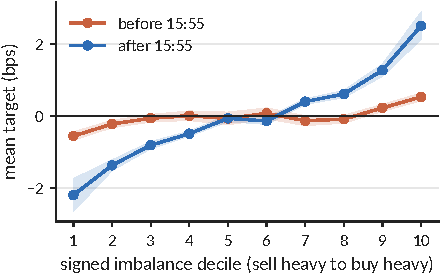
\includegraphics[width=\linewidth]{fig_decile_response}
  \caption{After 15:55 the imbalance sorts the next minute; before, it barely does. Every minute snapshot is ranked
  by signed imbalance and cut into ten equal groups, from the most sell-heavy (1) to the most buy-heavy (10). Each
  point is the group's mean move against the index. A fully priced imbalance would give a flat line at zero. Bands
  are 95\% intervals over days.}
  \label{fig:decile}
\end{figure}

\section{Statistical inferences}

\field{Rows tested:}{the \nTestRows{} snapshots at whole minutes (0, 60, \dots, 540\,s), so no two targets of a stock
overlap. Pre-15:55 rows are those at 0 to 240\,s, whose windows end by 15:55; post rows are those at 300 to 540\,s.
The unit of every primary test is the trading day ($n=\nDays$), because all stocks on a day share one index move.}

\field{Smallest difference that matters (SDM):}{the median quoted half-spread, \nSdm{} bps. The cheapest way to act
on the imbalance is to cross half the spread in the continuous book and exit in the closing cross, so a smaller edge
cannot be traded. Each test states its own threshold; all were fixed before testing.}

\field{Reading a result:}{an effect \emph{matters} when its whole 95\% interval lies beyond the threshold, and
\emph{does not matter} when the whole interval lies inside it. We use $\alpha=0.05$ per test and report Holm-adjusted
p-values across the six.}


\subsection*{Test 1 (P1): does the imbalance side predict the move?}

\tpart{a}{Hypotheses, written before running the test}
{\small
\begin{tabularx}{\linewidth}{@{}K{3.4cm} Y@{}}
\toprule
$H_0$ & $\mu\le0$ \\
$H_1$ & $\mu>0$ \\
Significance level & $\alpha=0.05$ \\
Side & one-sided (right) \\
Test & one-sample t-test on day means \\
Smallest difference that matters & \nSdm{} bps (the SDM) \\
\bottomrule
\end{tabularx}}

$\mu$ is the expected edge per trade, $E[\text{side}\times\text{target}]$, for a trader who buys on a buy imbalance
and sells on a sell imbalance. Each day gives one mean over its flagged snapshots. One-sided, because an efficient
market predicts zero and liquidity demand predicts a positive edge.

\tpart{b}{Other tests we considered}
Day means are independent across days and, by the CLT, close to normal at $n=\nDays$ even though rows are
heavy-tailed; $\sigma$ is unknown, so a one-sample t-test fits.\par
{\footnotesize
\begin{tabularx}{\linewidth}{@{}L{2.4cm} Y@{}}
\toprule
\textbf{Also considered} & \textbf{Why we did not use it} \\
\midrule
z-test on all rows & treats \nOneNaiveN{} rows as independent although each day shares one index move; it gives
$z=\nOneNaiveZ$, overstating the evidence. The \nOneOverlapN{} overlapping rows would be worse still \\
Welch t, buy vs sell rows & same question ($t=\nOneWelchT$, gap \nOneWelchDiff{} bps) with the same row dependence;
an F-test (ratio \nOneVarRatio) rules out the pooled t \\
Bootstrap over days & no normality needed; outside the syllabus, so a check: \nOneBootCi{} bps, same as the t interval \\
Permutation within snapshots & shuffles sides across stocks at each snapshot, \nPermOneN{} times; no shuffle came near
the observed edge (largest \nPermOneMax{} bps), p = \nPermOneP \\
\bottomrule
\end{tabularx}}

\tpart{c}{Result}
{\small
\begin{tabularx}{\linewidth}{@{}K{3.4cm} Y@{}}
\toprule
Estimate & $+\nOneEst$ bps per trade (raw target: $+\nOneRawEst$) \\
95\% confidence interval & \nOneCi{} bps \\
Test statistic (d.f.) & $t=\nOneT$ (\nOneDf) \\
p-value (Holm) & \nOneP{} (\nHolmOne) \\
Decision & reject $H_0$ \\
\bottomrule
\end{tabularx}}

The imbalance side predicts the next minute, on \nOnePositiveDays{} of \nDays{} days. The edge does not matter: even
the top of its interval is \nOneShareOfSdm{} of the half-spread, so the information is in the price to within trading
costs.

\subsection*{Test 2 (P1): is the direction of the move independent of the side?}

\tpart{a}{Hypotheses, written before running the test}
{\small
\begin{tabularx}{\linewidth}{@{}K{3.4cm} Y@{}}
\toprule
$H_0$ & side and direction are independent \\
$H_1$ & they are dependent \\
Significance level & $\alpha=0.05$ \\
Side & not applicable ($\chi^2$ is one-tailed by construction) \\
Test & $\chi^2$ test of independence, $3\times2$ table \\
Smallest difference that matters & Cramér's $V=\nTwoVThreshold$ \\
\bottomrule
\end{tabularx}}

Test 1 asks about the size of the move; Test 2 asks only about its sign, which is robust to the heavy tails. We use
the first snapshot of each stock-day (\nTwoN{} rows), so each stock appears once per day. $V=0.10$ is the conventional
floor for a small association.

\tpart{b}{Other tests we considered}
{\footnotesize
\begin{tabularx}{\linewidth}{@{}L{2.4cm} Y@{}}
\toprule
\textbf{Also considered} & \textbf{Why we did not use it} \\
\midrule
Two-proportion z-test & drops the balanced rows; on buy vs sell it gives $z=\nTwoPropZ$ and an up-share gap of
\nTwoDiff{} points (95\% CI \nTwoDiffCi) \\
G-test & same large-sample limit; $G=\nTwoG$, same decision \\
$\chi^2$ on all \nTwoAllN{} minute rows & repeats each stock nine more times a day, so rows are not independent;
$\chi^2=\nTwoAllChi$ \\
Paired t on daily gaps & dependence-robust check: $t=\nTwoDayT$, p = \nTwoDayP \\
\bottomrule
\end{tabularx}}

\tpart{c}{Result}
{\small
\begin{tabularx}{\linewidth}{@{}K{3.4cm} Y@{}}
\toprule
Estimate & $V=\nTwoV$; up-share \nTwoUpBuy{} after buy vs \nTwoUpSell{} after sell \\
Test statistic (d.f.) & $\chi^2=\nTwoChi$ (\nTwoDf) \\
p-value (Holm) & \nTwoP{} (\nHolmTwo) \\
Decision & reject $H_0$; smallest expected count \nTwoMinExpected \\
\bottomrule
\end{tabularx}}

The side and the direction are dependent, but weakly: $V$ is under a fifth of the smallest association that matters.

\minihead{What the central limit theorem buys us}
Test 1's interval relies on the CLT. Bounds from the lectures need weaker assumptions, at a price:

{\footnotesize
\begin{tabularx}{\linewidth}{@{}L{2.1cm} L{2.1cm} Y@{}}
\toprule
\textbf{Interval} & \textbf{Assumes} & \textbf{95\% interval for $\mu$ (bps)} \\
\midrule
t (CLT) & approx. normal day means & \nBoundTCi \\
Chebyshev & finite variance only & \nBoundChebCi{} (\nBoundChebRatio$\times$ wider) \\
Hoeffding & $|x|\le\nBoundRange$ bps & \nBoundHoeffCi{} (\nBoundHoeffRatio$\times$ wider) \\
\bottomrule
\end{tabularx}}

Chebyshev, which assumes almost nothing, still excludes zero and still sits below the SDM. Hoeffding uses only the
range, which the heavy tails make enormous, so it cannot even sign the effect.


\subsection*{Test 3 (P2): does a learned model see more than the imbalance?}

\tpart{a}{Hypotheses, written before training any model}
{\small
\begin{tabularx}{\linewidth}{@{}K{3.4cm} Y@{}}
\toprule
$H_0$ & $\mu_\Delta\le0$ \\
$H_1$ & $\mu_\Delta>0$ \\
Significance level & $\alpha=0.05$ \\
Side & one-sided (right) \\
Test & paired t-test over held-out days \\
Smallest difference that matters & $\Delta\text{IC}=\nSixThreshold$ \\
\bottomrule
\end{tabularx}}

We train on days 0 to 240, stop early on days 241 to 300, and test once on the \nSixTestDays{} days after that. A
two-layer MLP sees \nSixFeatures{} features of the auction state, including the recent path of prices and imbalance
but not the stock's identity. $\Delta_d$ is the MLP's daily IC minus the imbalance's daily IC on the same test day.
Each model is trained with five seeds and the predictions averaged.

\tpart{b}{Other tests we considered}
Both ICs of a day are computed on the same stocks and moves, so they are paired.\par
{\footnotesize
\begin{tabularx}{\linewidth}{@{}L{2.4cm} Y@{}}
\toprule
\textbf{Also considered} & \textbf{Why we did not use it as primary} \\
\midrule
Diebold-Mariano & compares squared forecast errors, not rankings; MLP vs a linear imbalance forecast gives
$t=\nDmLinT$, same decision \\
Sign-flip permutation & distribution-free check on $\Delta_d$; p = \nSixPerm \\
LightGBM, GRU & alternative learners, not alternative tests: LightGBM IC \nLgbmIc, GRU \nGruIc{}; the MLP was fixed
as primary in advance \\
z-test on all test rows & treats \nSixTestRows{} rows as independent, ignoring the shared index move of a day \\
\bottomrule
\end{tabularx}}

\tpart{c}{Result}
{\small
\begin{tabularx}{\linewidth}{@{}K{3.4cm} Y@{}}
\toprule
Estimate & $\Delta\text{IC}=+\nSixEst$ (MLP \nSixMlp, imbalance \nSixBase) \\
95\% confidence interval & \nSixCi \\
Test statistic (d.f.) & $t=\nSixT$ (\nSixDf) \\
p-value (Holm) & \nSixP{} (\nHolmSix) \\
Decision & reject $H_0$ \\
\bottomrule
\end{tabularx}}

On the official target the MLP ranks next-minute moves \nSixRatio{} times better than the imbalance, and five seeds
agree to within \nSeedSdMlp{} in IC. Figure~\ref{fig:cumic} shows the catch.

\begin{figure}[!t]
  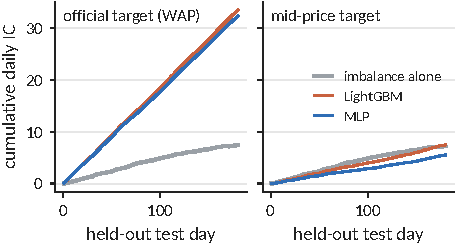
\includegraphics[width=\linewidth]{fig_cumulative_ic}
  \caption{The learned gain is an artefact of how the target is built. Left: on the official target, which is
  computed from the size-weighted mid (WAP), both models leave the imbalance far behind. Right: on the plain
  mid-price move of the same rows, the imbalance alone is at least as good. Lines add up each test day's IC.}
  \label{fig:cumic}
\end{figure}

\minihead{The learned gain is WAP mechanics (check fixed before the five-seed run)}
The official target is a return of the WAP, which shifts toward the thinner side of the book whenever depth changes.
A model that reads depth can therefore predict the WAP without predicting the price; depth imbalance is indeed the
model's most used feature (\nImpFirstShare{} of LightGBM's split gain). Re-scored against the plain mid-price
move, the MLP's IC falls to \nMidMlp{} while the imbalance keeps \nMidBase{}: the gain becomes \nMidGain{} (95\% CI
\nMidGainCi). By the rule we fixed before the run, most of the learned gain is WAP mechanics. The imbalance itself
passes the same check: its Test 1 edge is \nWapOneEst{} bps on the WAP and \nMidOneEst{} bps on the mid over the same
rows.

\subsection*{Test 4 (P3): does 15:55 change how predictable the move is?}

\tpart{a}{Hypotheses, written before running the test}
{\small
\begin{tabularx}{\linewidth}{@{}K{3.4cm} Y@{}}
\toprule
$H_0$ & $\mu_\Delta=0$ \\
$H_1$ & $\mu_\Delta\neq0$ \\
Significance level & $\alpha=0.05$ \\
Side & two-sided \\
Test & paired t-test over days \\
Smallest difference that matters & $|\Delta\text{IC}|=\nThreeThreshold$ \\
\bottomrule
\end{tabularx}}

The information coefficient (IC) is the rank correlation, across stocks, between signed imbalance and the next move:
0 means no predictive power, 1 a perfect ranking. Each day gives an IC before and after 15:55, and $\Delta_d$ is
post minus pre. Two-sided, because the near price could absorb the imbalance information or sharpen it. A change of
0.02 is of the same order as the IC itself.

\tpart{b}{Other tests we considered}
The two ICs of a day come from the same stocks in the same market, so they are paired; the paired t-test removes the
day effect.\par
{\footnotesize
\begin{tabularx}{\linewidth}{@{}L{2.4cm} Y@{}}
\toprule
\textbf{Also considered} & \textbf{Why we did not use it} \\
\midrule
Fisher z on two pooled correlations & assumes two independent samples, but they share stocks and days; gives
$z=\nThreeFisherZ$ \\
t-test for each correlation & tests each phase against zero, not the change; pre $r=\nThreePooledPre$
($t=\nThreePooledPreT$), post $r=\nThreePooledPost$ ($t=\nThreePooledPostT$) \\
Sign test over days & distribution-free; \nThreeSignDays{} of \nDays{} days rise, p = \nThreeSignP \\
Sign-flip permutation & randomly swaps each day's pre and post, \nFlipThreeN{} times; largest \nFlipThreeMax, p =
\nFlipThreeP \\
\bottomrule
\end{tabularx}}

\tpart{c}{Result}
{\small
\begin{tabularx}{\linewidth}{@{}K{3.4cm} Y@{}}
\toprule
Estimate & $\Delta\text{IC}=+\nThreeEst$ (IC \nThreePre{} before, \nThreePost{} after) \\
95\% confidence interval & \nThreeCi \\
Test statistic (d.f.) & $t=\nThreeT$ (\nThreeDf) \\
p-value (Holm) & \nThreeP{} (\nHolmThree) \\
Decision & reject $H_0$ \\
\bottomrule
\end{tabularx}}

The imbalance predicts the next minute \nThreeRatio{} times better after 15:55, and the whole interval lies beyond
the threshold. We had predicted, in writing, a fall. The placebo test after Test 5 shows where the rise really comes from.

\subsection*{Test 5 (P3): is the next minute less volatile after 15:55?}

\tpart{a}{Hypotheses, written before running the test}
{\small
\begin{tabularx}{\linewidth}{@{}K{3.4cm} Y@{}}
\toprule
$H_0$ & $\sigma^2_{\text{post}}/\sigma^2_{\text{pre}}=1$ \\
$H_1$ & $\sigma^2_{\text{post}}/\sigma^2_{\text{pre}}\neq1$ \\
Significance level & $\alpha=0.05$ \\
Side & two-sided \\
Test & F-test for two variances \\
Smallest difference that matters & ratio outside \nFourLow{} to \nFourHigh{} \\
\bottomrule
\end{tabularx}}

A 10\% change in variance is a 5\% change in volatility, the scale at which a market maker would re-price quotes.

\tpart{b}{Other tests we considered}
The F-test is the syllabus test for two variances, but it assumes normal data and our target has excess kurtosis of
\nFourKurtPre{} before and \nFourKurtPost{} after 15:55. We read it beside two checks that do not need normality.\par
{\footnotesize
\begin{tabularx}{\linewidth}{@{}L{2.4cm} Y@{}}
\toprule
\textbf{Also considered} & \textbf{Why we did not use it as primary} \\
\midrule
Brown-Forsythe & robust to heavy tails; $W=\nFourBf$, p \nFourBfP, same decision \\
t on daily log variance ratio & respects day dependence; ratio \nFourDayRatio{} (95\% CI \nFourDayRatioCi),
$t=\nFourDayT$ \\
$\chi^2$ for one variance & needs a known $\sigma_0$; we compare two unknown variances \\
\bottomrule
\end{tabularx}}

\tpart{c}{Result}
{\small
\begin{tabularx}{\linewidth}{@{}K{3.4cm} Y@{}}
\toprule
Estimate & $F=\nFourF$ (sd \nFourSdPre{} to \nFourSdPost{} bps) \\
95\% confidence interval & \nFourCi \\
Test statistic (d.f.) & $F=\nFourF$ (\nFourDf, \nFourDf) \\
p-value (Holm) & \nFourP{} (\nHolmFour) \\
Decision & reject $H_0$ \\
\bottomrule
\end{tabularx}}

The next minute is about \nFourDrop{} less variable after 15:55, and all three tests agree, including the two that do
not assume normality. The change matters: the interval lies below \nFourLow.

\minihead{Is 15:55 really the cause? Placebo boundaries (P3)}
If the rule change drives Test 4, the IC should jump at 15:55 and nowhere else. The jump at 15:55 is real,
$+\nJumpReal$ (95\% CI \nJumpRealCi), but the jump into the last minute is larger, $+\nJumpLast$ (\nJumpLastCi), so
our pre-set criterion fails.

\begin{figure}[!t]
  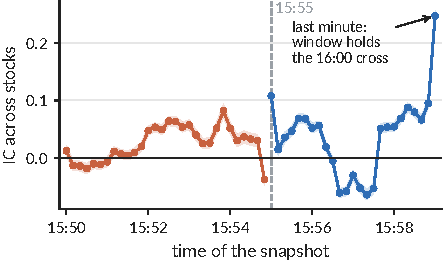
\includegraphics[width=\linewidth]{fig_ic_profile}
  \caption{Predictability is not a step at 15:55: it spikes for one snapshot at 15:55, fades, turns negative near
  15:57, and peaks in the last minute, whose window contains the 16:00 closing cross. Each point is the IC across
  stocks at one 10\,s snapshot, averaged over days, with a 95\% band.}
  \label{fig:icprofile}
\end{figure}

Figure~\ref{fig:icprofile} shows why. The IC leaps from \nIcBeforeBoundary{} to \nIcAtBoundary{} across 15:55, fades
to \nIcMin{} near 15:57, and reaches \nIcLast{} for the last minute. Dropping that minute shrinks the post-minus-pre
gain from \nSensWith{} (\nSensWithCi) to \nSensWithout{} (\nSensWithoutCi), inside our threshold. Publishing the near
price causes a brief spike; the lasting gain is the imbalance telling us about the closing print itself. We label
this decomposition exploratory, since it came after the placebo result. The rise itself is positive in all
\nRobPositive{} of \nRobTotal{} subgroups we fixed in advance (by period, size, spread and day volatility), and a
classifier tells pre- from post-15:55 auction states apart with \nCtAcc{} accuracy on held-out days.

\subsection*{Test 6 (P4): can an outsider trade the imbalance?}

\tpart{a}{Hypotheses, written before running the test}
{\small
\begin{tabularx}{\linewidth}{@{}K{3.4cm} Y@{}}
\toprule
$H_0$ & $p\le0.5$ \\
$H_1$ & $p>0.5$ \\
Significance level & $\alpha=0.05$ \\
Side & one-sided (right) \\
Test & one-proportion z-test \\
Smallest difference that matters & $p=\nFiveThreshold$ \\
\bottomrule
\end{tabularx}}

$p$ is the chance that a trade in the imbalance direction earns more than its own half-spread. A rule that wins
52\% of the time is a two-point edge over a coin.

\tpart{b}{Other tests we considered}
{\footnotesize
\begin{tabularx}{\linewidth}{@{}L{2.4cm} Y@{}}
\toprule
\textbf{Also considered} & \textbf{Why we did not use it} \\
\midrule
Exact binomial & identical at $n=\nFiveN$; same decision \\
t on daily hit rates & dependence-robust check; $t=\nFiveDayT$ \\
Mean net P\&L & Test 1 already tests the mean; a rate is what a trader monitors \\
\bottomrule
\end{tabularx}}

\tpart{c}{Result}
{\small
\begin{tabularx}{\linewidth}{@{}K{3.4cm} Y@{}}
\toprule
Estimate & $\hat p=\nFiveEst$ (\nFiveGross{} before costs) \\
95\% confidence interval & \nFiveCi{}\% \\
Test statistic & $z=\nFiveZ$ \\
p-value (Holm) & \nFiveP{} (\nHolmFive) \\
Decision & fail to reject $H_0$ \\
\bottomrule
\end{tabularx}}

Before costs the rule wins slightly more than half the time; after paying the half-spread it wins only \nFiveEst,
and the average trade loses \nFiveNet{} bps. On the mid price the hit rate is
\nMidFiveHit{}, so the verdict does not depend on how the target is built.

\minihead{Who can trade it? Edge against cost (P4)}
Figure~\ref{fig:edge} sets the average edge per trade against the half-spread at every snapshot. The edge stays
below the cost for the whole auction except the last minute. Trading only the strongest tenth of imbalances after
15:55 raises the gross edge to \nStrongGross{} bps, but those stocks quote a half-spread of \nStrongHalf, so the net
is \nStrongNet{} bps (\nStrongNetCi). Strong imbalances appear exactly where trading is expensive.

\begin{figure}[!t]
  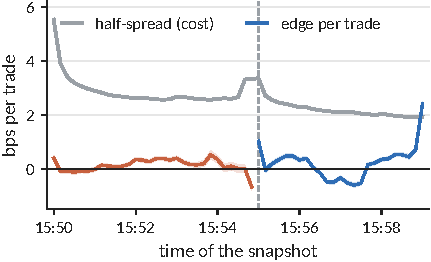
\includegraphics[width=\linewidth]{fig_edge_vs_cost}
  \caption{The imbalance edge (coloured, with 95\% band) never covers the half-spread (grey) until the last minute.
  Each point averages, over days, the gross edge of trading in the imbalance direction at that snapshot.}
  \label{fig:edge}
\end{figure}

The learned model does not change this. Trading only when the MLP's forecast exceeds the half-spread appears to earn
\nSelNet{} bps per trade on the WAP target, but \nSelMidNet{} bps (\nSelMidNetCi) on the mid price, a loss. At the
15:59 snapshot, and only there, the imbalance edge of \nFinalGross{} bps beats a half-spread of \nFinalHalf, a net
\nFinalNet{} bps (\nFinalNetCi) that shrinks from \nFinalFirst{} in the first half of the days to \nFinalSecond{} in the
second. We found it after looking, and it ignores the cost of hedging the index and of getting filled, so it is a lead
for future work, not a result.

\minihead{Answers}
{\footnotesize
\begin{tabularx}{\linewidth}{@{}L{0.7cm} Y@{}}
\toprule
P1 & Yes. The imbalance predicts the next minute on \nOnePositiveDays{} of \nDays{} days, in real price moves, not
only in the WAP. \\
P2 & Only on paper. The learned gain on the official target is WAP mechanics; on the mid price the imbalance alone
is as good. \\
P3 & Partly. Predictability and volatility change after 15:55, but the lasting gain is the closing cross, not the
rule. \\
P4 & No, except possibly in the last minute, an exploratory lead. The information is in the price to within trading
costs. \\
\bottomrule
\end{tabularx}}

\section{Limitations}

\begin{itemize}
  \item \textbf{Two rules change at once, next to the close.} At 15:55 the near price appears and market-on-close
  entry closes; the placebo test shows the post-15:55 gain is mostly the final minute, so time to the close and the
  rule change are not separated.
  \item \textbf{Association, not cause.} The imbalance may predict because the same traders move both, not because
  traders read it.
  \item \textbf{Days treated as independent.} Market-wide news can link consecutive days; the effects are large
  enough that modest dependence would not change a decision.
  \item \textbf{One model family, one split.} P2 uses one MLP design and one chronological split; a different
  architecture could find real price information we did not.
  \item \textbf{Costs are approximate.} The half-spread is a snapshot quote; fees, impact, index hedging and auction
  fills are not modelled, so the true cost is higher.
  \item \textbf{One exchange, anonymised period.} Dates and tickers are hidden, so results cover these 200 Nasdaq
  stocks over about two years.
\end{itemize}

Supplementary material (figures and tables for every check above, the full pre-registration log and the model
settings) is in \code{report/supplementary.pdf} in the code repository.

\end{document}
